\documentclass[11pt]{article}

%------------------------- Packages -------------------------
\usepackage[margin=1in]{geometry}
\usepackage{amsmath, amssymb}
\usepackage{graphicx}
\usepackage{listings}
\usepackage[hidelinks]{hyperref}
\usepackage{enumitem}
\usepackage{indentfirst}
\usepackage{titling}

% Figures are resolved from results/figures/ (this file lives in results/reports/).
\graphicspath{{../figures/}}

%------------------------- Paragraph indentation -------------------------
\setlength{\parindent}{2em}
\setlength{\parskip}{0pt plus 1pt}
\setlength{\droptitle}{-1.75cm}

%------------------------- Code style -------------------------
\lstset{
    basicstyle=\ttfamily\small,
    breaklines=true,
    frame=single
}

\title{\textbf{Lab3 Report}}
\author{}
\date{}

\begin{document}
\maketitle

\section*{Task 1}

We implement the ring (1D-torus) topology and a minimal adaptive ring routing
algorithm. \texttt{Ring.py} under \texttt{configs/topologies} arranges the 16
routers in a closed loop: every router has two bidirectional internal links,
one leaving via the \texttt{Right} outport into the right neighbour's
\texttt{Left} inport and one leaving via \texttt{Left} into the left
neighbour's \texttt{Right} inport; external links attach each controller to
its router, as in \texttt{Mesh\_XY}. A new routing-algorithm id
(\texttt{RING\_ = 3}) is registered and dispatched by
\texttt{RoutingUnit::outportComputeRing()}: for a packet from router $s$ to
router $d$ it computes the clockwise distance $\delta_R = (d-s) \bmod 16$ and
the counter-clockwise distance $\delta_L = (s-d) \bmod 16$, then picks the
shorter direction (ties go to \texttt{Right}). Because this minimal route uses
both directions of the loop, the channel-dependency graph contains a
wrap-around cycle, so the single-VC ring deadlocks once the offered load fills
the loop.

The results are shown in Figure~\ref{fig:task1}. Because of the special
structure of \texttt{bit\_complement} on the ring (each node $i$ exchanges
with its mirror node $15-i$), its traffic leaves ``holes'' in the loop, so it
never actually deadlocks within the tested range. However, once the injection
rate exceeds $0.25$ the network becomes heavily congested: the queueing
latency explodes to thousands of cycles and the accepted throughput is pinned
at $\approx 0.25$ flits/cycle/node, so the network keeps delivering packets but
with very low efficiency.

At low load, before any deadlock, the three metrics compare as follows. The
average hop count is fixed by the traffic pattern: \texttt{bit\_reverse}
travels $\approx 3.74$ hops, while \texttt{uniform\_random} and
\texttt{bit\_complement} both average $\approx 4.0$ hops, and the low-load
latency follows the same ordering. The link utilization grows almost linearly
with the injection rate for all three patterns and is nearly equal at the same
rate, since it is proportional to $\text{throughput} \times (\text{hops}+2)$.

\begin{figure}[htbp]
    \centering
    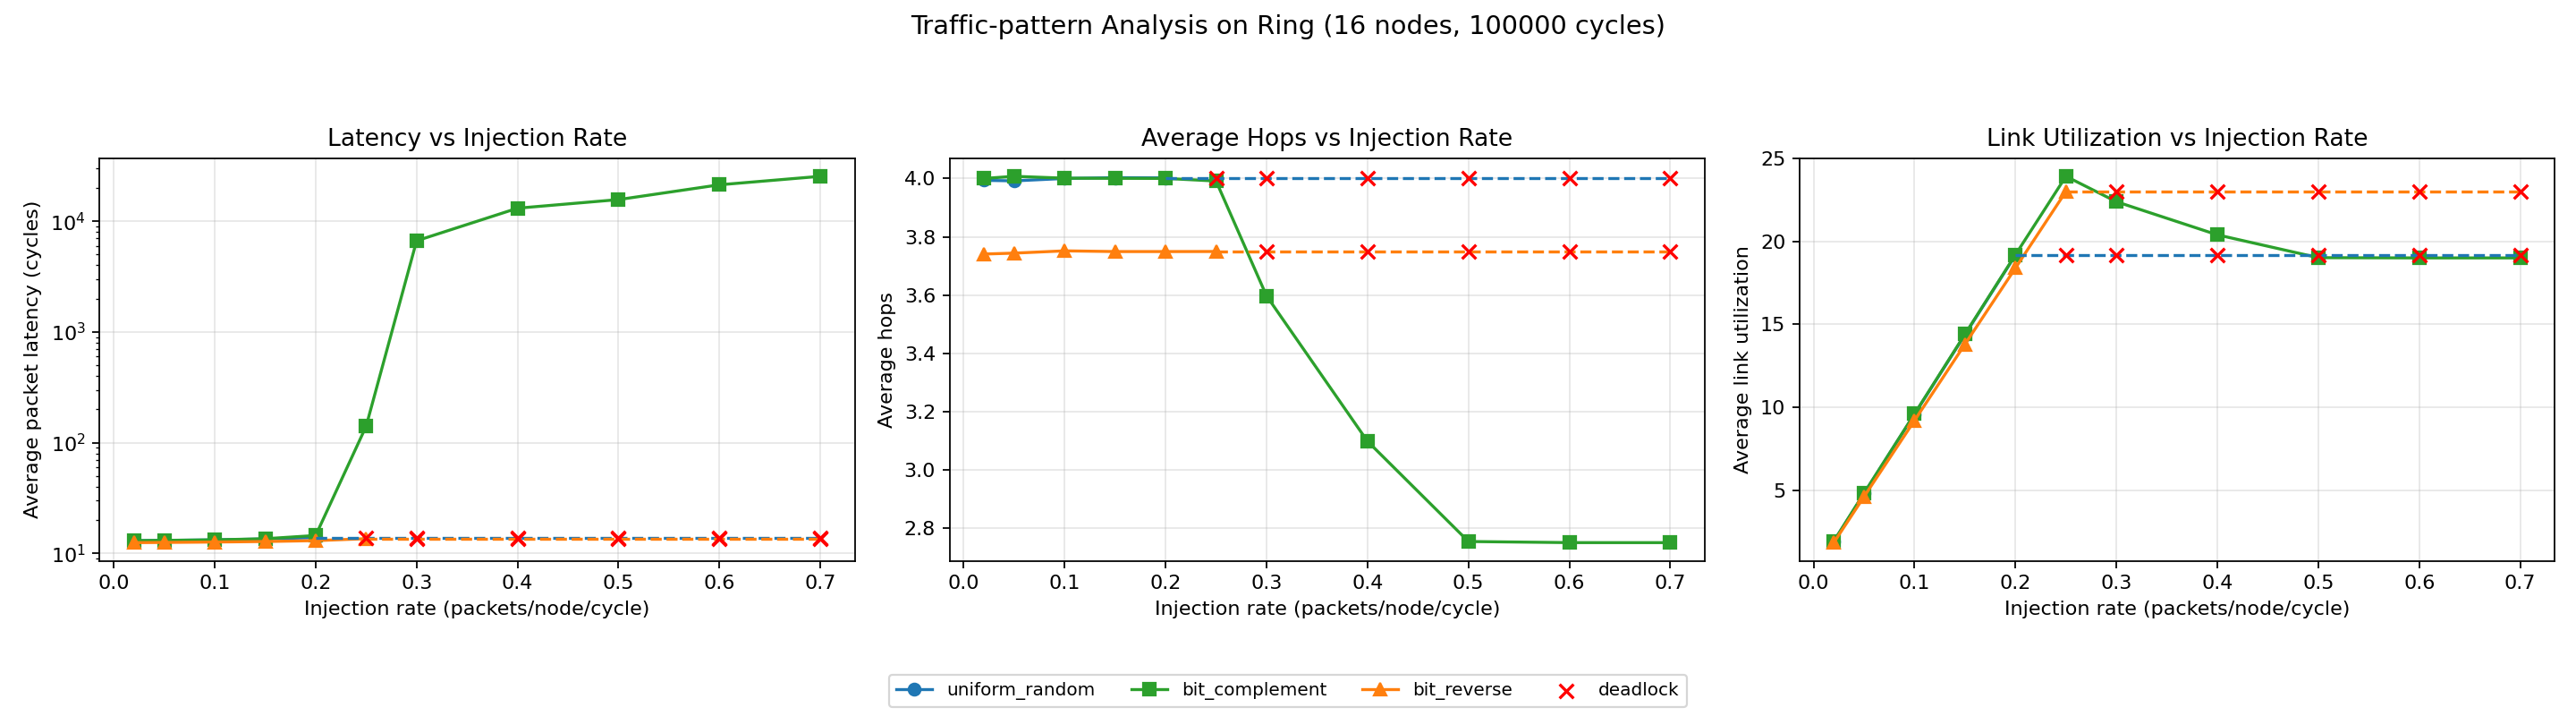
\includegraphics[width=0.9\textwidth]{lab3_task1_analysis.png}
    \caption{Ring topology (16 nodes, ring routing): latency (log scale),
    average hops, and link utilization versus injection rate. Red crosses
    mark deadlocked runs.}
    \label{fig:task1}
\end{figure}

\section*{Task 2}

By default each virtual channel (VC) holds exactly one packet. We add a
\texttt{--wormhole} option that lets every VC hold up to
\texttt{WORMHOLE\_DEPTH = 16} single-flit packets, and evaluate it against two
credit-based baselines on the ring:
\begin{itemize}[itemsep=1pt, topsep=2pt]
    \item \textbf{VC = 1, Depth = 1} (\texttt{--vcs-per-vnet=1}): one
    single-flit slot per VC;
    \item \textbf{VC = 16, Depth = 1} (\texttt{--vcs-per-vnet=16}): 16
    independent single-packet VCs;
    \item \textbf{VC = 1, Depth = 16} (\texttt{--vcs-per-vnet=1 --wormhole}):
    one VC acting as a 16-slot FIFO.
\end{itemize}
All runs inject single-flit packets (\texttt{--inj-vnet=0}, so
\texttt{t\_flit->get\_type() == HEAD\_TAIL\_}) into a 16-node ring with ring
routing. The key implementation points: \texttt{OutVcState} advertises 16
buffer credits instead of the per-VC depth; \texttt{InputUnit} performs route
computation per flit (each single-flit packet stores its own output port) and
allows a \texttt{HEAD\_TAIL} flit to arrive into an already-active VC;
\texttt{OutputUnit}/\texttt{SwitchAllocator} select an output VC as long as it
still has a free buffer slot; and \texttt{NetworkInterface} keeps injecting
into the same VC while credits remain.

The three traffic patterns are shown in Figures~\ref{fig:task2_uniform},
\ref{fig:task2_complement} and \ref{fig:task2_reverse}. First, as already
observed in Task 1, \texttt{bit\_complement} does not deadlock in any of the
three configurations: its mirrored pairing leaves ``holes'' in the ring, so the
wrap-around cycle never fully closes; it merely saturates.

The central result is that the \textbf{VC = 16, Depth = 1} and \textbf{wormhole}
(VC = 1, Depth = 16) configurations are indistinguishable: their latency,
throughput, hop count and deadlock points all match. The reason is that with
single-flit packets each buffer slot holds exactly one flit, so both
configurations provide the same 16 slots of buffering per virtual network and
--- because the wormhole switch allocator treats every flit independently ---
the same freedom from head-of-line blocking. What matters is therefore the
total buffer capacity per vnet, not how that capacity is partitioned into VCs.

The meaningful contrast is between \textbf{depth 16} and \textbf{depth 1}
(VC = 1). At low load they behave alike (same hop count, nearly the same
latency), with depth 1 only slightly slower because its single-slot VC forces
the network interface to wait for a credit round-trip before injecting again.
At high load they diverge sharply: \textbf{VC = 1, Depth = 1} deadlocks at
$0.04$ (\texttt{uniform\_random}) and $0.075$ (\texttt{bit\_reverse}), and for
\texttt{bit\_complement} it saturates already at $0.075$ with the throughput
stuck at $\approx 0.0625$ flits/cycle/node. In contrast, \textbf{depth 16}
tracks the offered load up to rate $0.3$ (throughput $\approx 0.3$
flits/cycle/node) for \texttt{uniform\_random} and \texttt{bit\_reverse} and
deadlocks only at $0.4$, while for \texttt{bit\_complement} it never deadlocks
up to $0.7$ and merely saturates around $0.25$. In short, for single-flit
traffic, buffer depth --- not the number of VCs --- is what provides deadlock
freedom and bandwidth.

\begin{figure}[htbp]
    \centering
    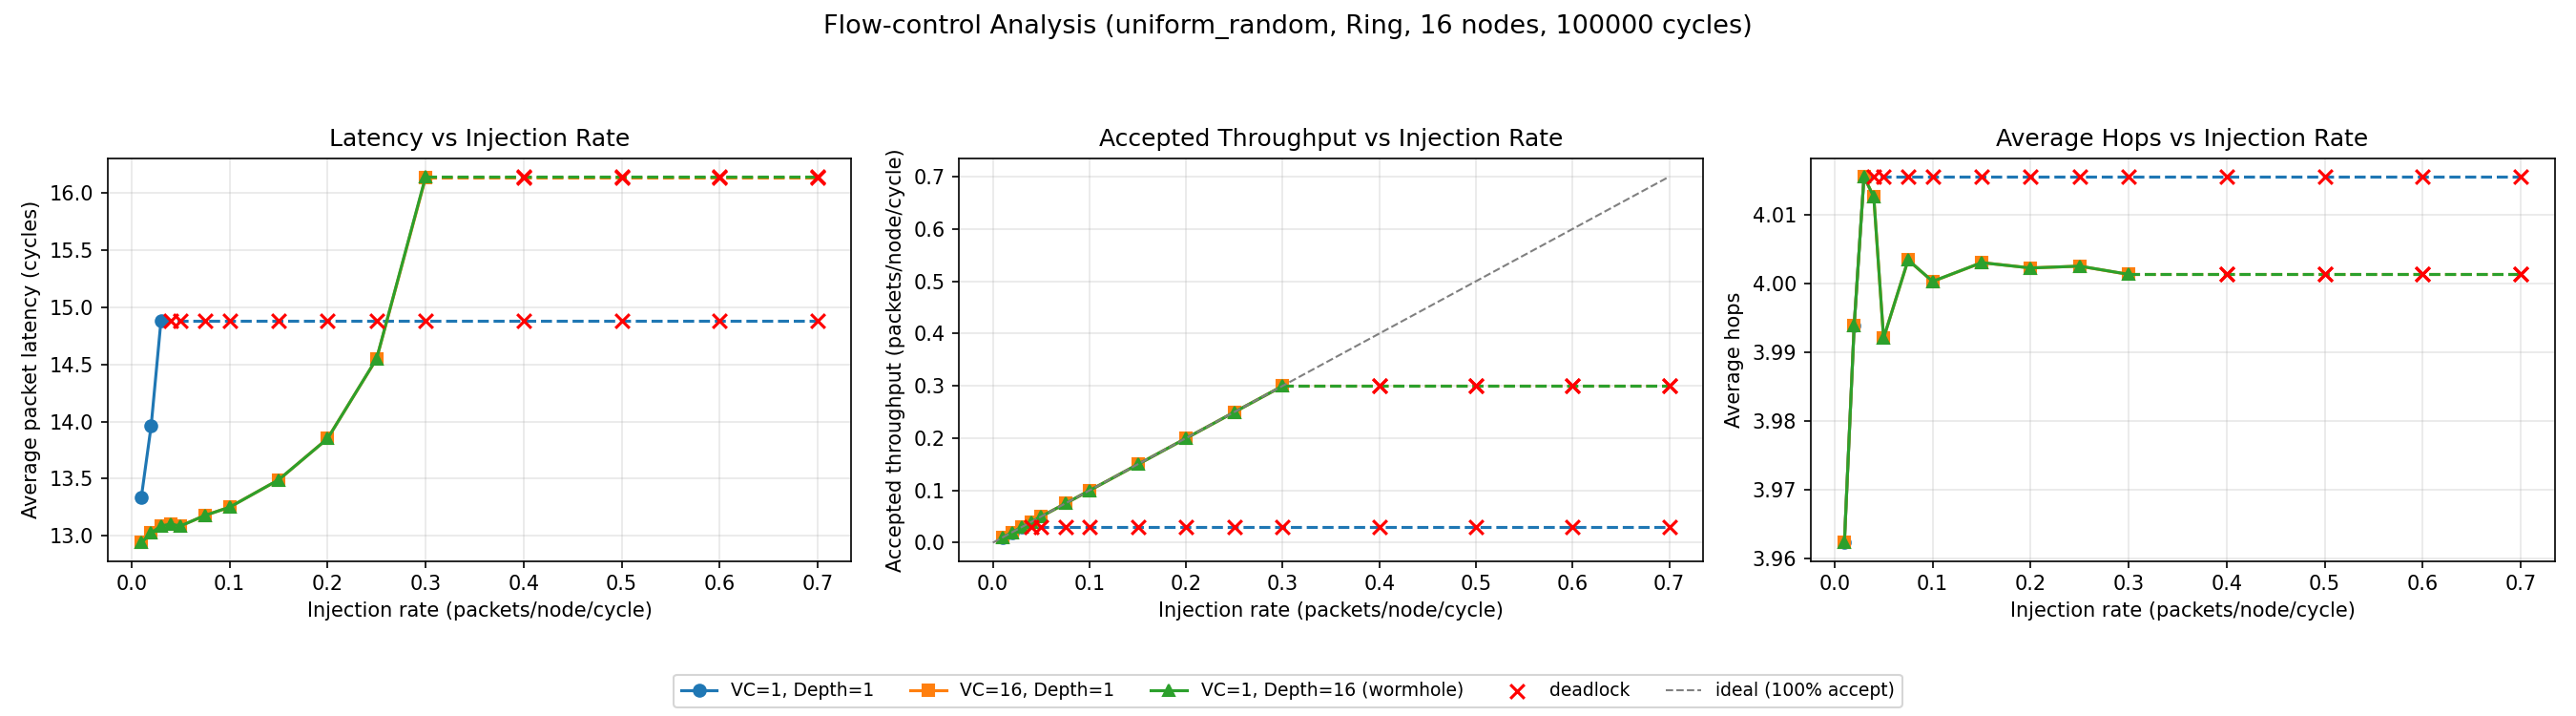
\includegraphics[width=0.9\textwidth]{lab3_task2_uniform_random_analysis.png}
    \caption{Flow-control comparison under \texttt{uniform\_random} traffic:
    latency, accepted throughput, and average hops versus injection rate.
    Red crosses mark deadlocked runs.}
    \label{fig:task2_uniform}
\end{figure}
\begin{figure}[htbp]
    \centering
    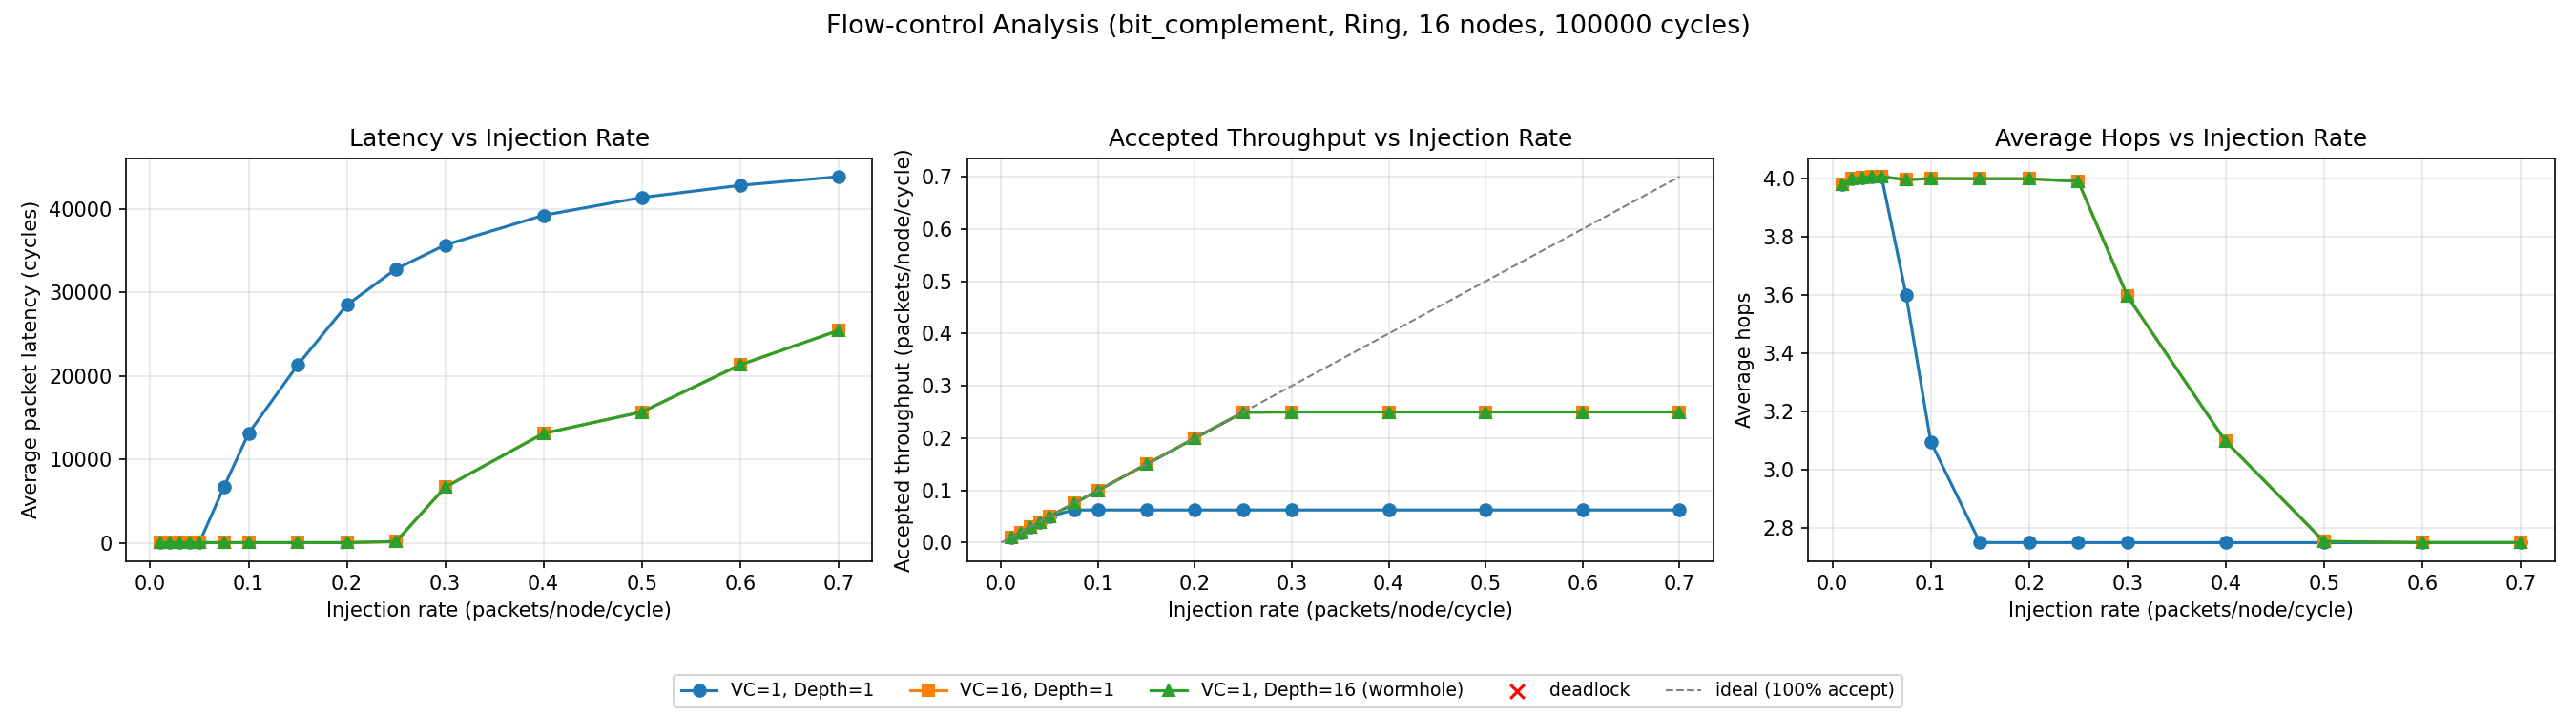
\includegraphics[width=0.9\textwidth]{lab3_task2_bit_complement_analysis.png}
    \caption{Flow-control comparison under \texttt{bit\_complement} traffic.}
    \label{fig:task2_complement}
\end{figure}
\begin{figure}[htbp]
    \centering
    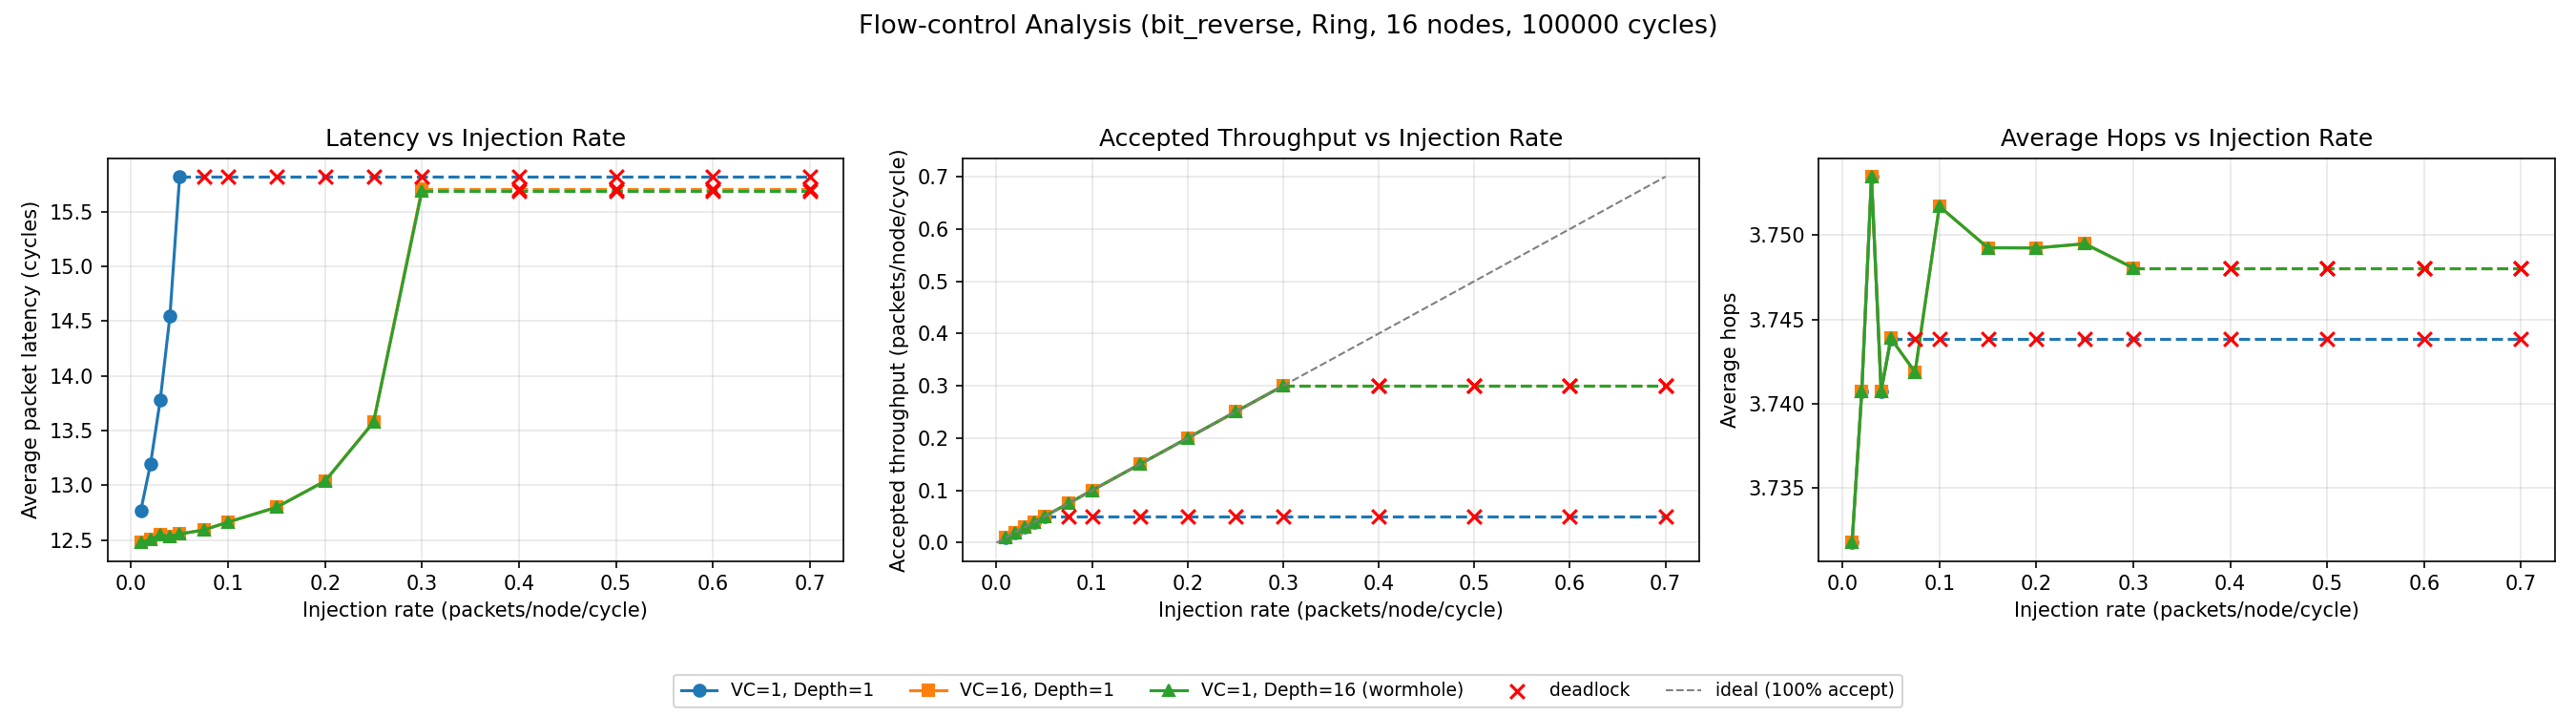
\includegraphics[width=0.9\textwidth]{lab3_task2_bit_reverse_analysis.png}
    \caption{Flow-control comparison under \texttt{bit\_reverse} traffic.}
    \label{fig:task2_reverse}
\end{figure}

\end{document}
